\documentclass[tikz]{standalone}
\usepackage{pgfplots}

\pgfplotsset{compat=newest}
\pgfplotsset{
    yticklabel style={
        /pgf/number format/fixed,
        /pgf/number format/precision=2
    },
    scaled y ticks=false
}

\begin{document}
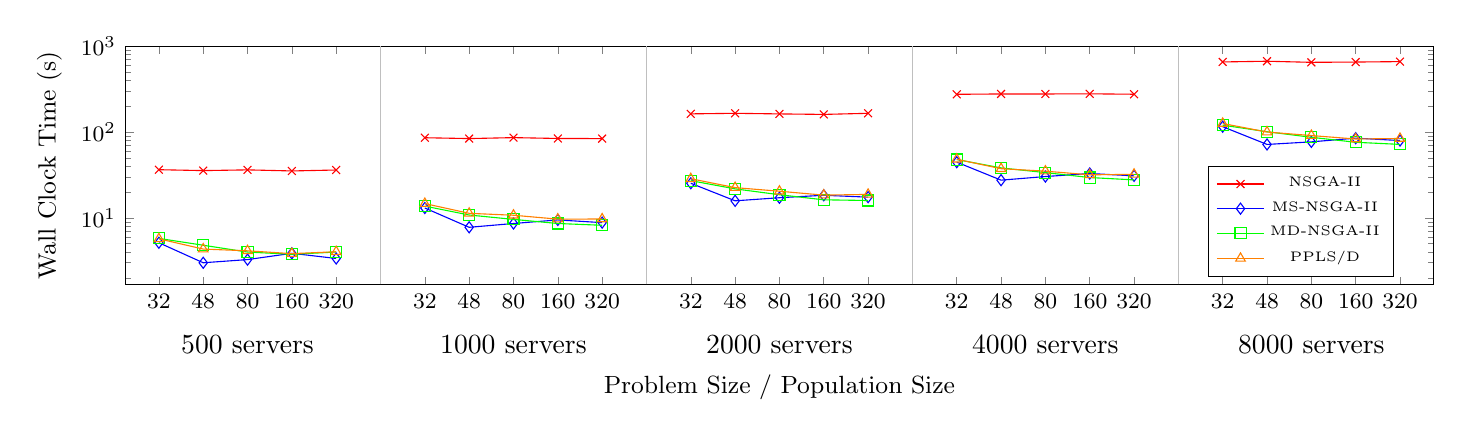
\begin{tikzpicture}

    \begin{axis}[
        footnotesize,
        max space between ticks=20pt,
        width=1.5\textwidth,
        height=0.38\textwidth,
        ymax = 1000,
        try min ticks=5,
        xtick=data,
        xticklabels={32, 48, 80, 160, 320, 32, 48, 80, 160, 320, 32, 48, 80, 160, 320, 32, 48, 80, 160, 320, 32, 48, 80, 160, 320},
        extra x ticks={5,11,17,23},
        extra x tick labels={},
        extra x tick style={
            grid=major,
            major tick length=0pt,
        },
        xlabel={Problem Size / Population Size},
        ylabel={Wall Clock Time (s)},
        xlabel style={
            yshift=-4ex,
        },
        enlarge x limits={abs=0.75},
        legend pos=south east,
        legend entries={
            {NSGA-II},
            {MS-NSGA-II},
            {MD-NSGA-II},
            {PPLS/D},
        },
        clip mode=individual,
        legend style={font=\tiny},
        ymode=log,
    ]

    \addplot[
        mark=x,
        color=red
    ] table[
        x expr=\coordindex,
        y=TM
    ]{
        PS TM
        32 36.4
        48 35.5333
        80 36.2333
        160 35.2
        320 36.1
        {} {}
        
        32 85.7667
        48 83.8667
        80 86.0333
        160 84.1
        320 83.8333
        {} {}
        
        32 162.7333
        48 165.1333
        80 162.5
        160 160.3333
        320 165.1333
        {} {}
        
        32 274.9
        48 277.5
        80 277.3333
        160 278.4667
        320 275.4333
        {} {}
        
        32 654.8667
        48 667.3333
        80 648.1
        160 653.0333
        320 660.6333
        {} {}            
    };

    \addplot[
        mark=diamond,
        color=blue
    ] table[
        x expr=\coordindex,
        y=TM
    ]{
        PS TM
        32 5.1333
        48 3
        80 3.2667
        160 3.8667
        320 3.3667
        {} {}
        
        32 13.0333
        48 7.7667
        80 8.6
        160 9.4667
        320 8.8
        {} {}
        
        32 25.3
        48 15.8
        80 17.1667
        160 18.3333
        320 17.4333
        {} {}
        
        32 44.5667
        48 27.5
        80 30.3
        160 32.8667
        320 30.8667
        {} {}
        
        32 115.3667
        48 71.6667
        80 76.8
        160 84.8333
        320 79.5667
        {} {}           
    };

    \addplot[
        mark=square,
        color=green
    ] table[
        x expr=\coordindex,
        y=TM
    ]{
        PS TM
        32 5.7667
        48 4.8
        80 4
        160 3.7667
        320 4
        {} {}
        
        32 13.7
        48 10.8
        80 9.6
        160 8.6
        320 8.2
        {} {}
        
        32 27.1333
        48 21.7667
        80 18.6
        160 16.2333
        320 15.9333
        {} {}
        
        32 47.8
        48 38.2
        80 33.6667
        160 29.5
        320 27.7
        {} {}
        
        32 120.2333
        48 100.7333
        80 86.8
        160 75.9333
        320 71.7667
        {} {}                        
    };

    \addplot[
        mark=triangle,
        color=orange
    ] table[
        x expr=\coordindex,
        y=TM
    ]{
        PS TM
        32 5.7
        48 4.3333
        80 4.1333
        160 3.8333
        320 4.0333
        {} {}
        
        32 14.6667
        48 11.3
        80 10.7333
        160 9.6667
        320 9.7
        {} {}
        
        32 28.5667
        48 22.5
        80 20.4333
        160 18.4
        320 18.7667
        {} {}
        
        32 48.1333
        48 37.4
        80 35
        160 31.7333
        320 32.1333
        {} {}
        
        32 125.6333
        48 99.9333
        80 90.9333
        160 82.9
        320 84.0667
        {} {}           
    };

    \begin{scope}[
        every label/.append style={
            label distance=2ex,
        },
    ]
        \node [label=below:500 servers, yshift=3ex]
            at (axis cs:2,\pgfkeysvalueof{/pgfplots/ymin}) {};
        \node [label=below:1000 servers, yshift=3ex]
            at (axis cs:8,\pgfkeysvalueof{/pgfplots/ymin}) {};
        \node [label=below:2000 servers, yshift=3ex]
            at (axis cs:14,\pgfkeysvalueof{/pgfplots/ymin}) {};
        \node [label=below:4000 servers, yshift=3ex]
            at (axis cs:20,\pgfkeysvalueof{/pgfplots/ymin}) {};
        \node [label=below:8000 servers, yshift=3ex]
            at (axis cs:26,\pgfkeysvalueof{/pgfplots/ymin}) {};
    \end{scope}
    \end{axis}
\end{tikzpicture}
\end{document}